\documentclass{beamer}
\usepackage[english]{babel}
\usepackage[utf8x]{inputenc}
\usepackage[IL2]{fontenc}
\usepackage{lmodern}


\mode<presentation> {

\AtBeginSection[]
{
  \begin{frame}<beamer>
%     \frametitle{Outline for section \thesection}
    \frametitle{Outline}
    \tableofcontents[currentsection]
  \end{frame}
}


  \usetheme{Warsaw}
%    \usetheme{CambridgeUS}
  \setbeamercovered{transparent}
  \setbeamertemplate{navigation symbols}{} 
  \useoutertheme{infolines} 
}



\usepackage{ucs}
% \usepackage{palatino}
\usepackage{graphicx}



\usepackage{multirow}
\usepackage{hyperref}
\usepackage{color}
\usepackage{afterpage}
\usepackage{calc}
%\usepackage{subfig}
\usepackage{amssymb}
\usepackage{amsthm}
\usepackage{amsmath}
% \usepackage{enumitem}
%\usepackage{titlesec}

% floating for figures H
%\usepackage{float}
%\restylefloat{figure}

\usepackage{fixltx2e}		% text super/sub scripts
%\usepackage{algpseudocode}
%\usepackage{algorithm}

\usepackage{units} 		% nicefrac

\newtheorem{mydef}{Definition}
\newtheorem{myprop}{Proposition}
\newtheorem{mytheorem}{Theorem}
\newcommand{\gfe}{\ensuremath{\text{GF}\left(2^8\right)}}
\newcommand{\gf}{\ensuremath{\text{GF}\left(2\right)}}

\usepackage[absolute,overlay]{textpos}
\setbeamercolor{framesource}{fg=gray}
\setbeamerfont{framesource}{size=\tiny}

\newcommand{\source}[1]{\begin{textblock*}{4cm}(8.7cm,8.6cm)
    \begin{beamercolorbox}[ht=0.5cm,right]{framesource}
        \usebeamerfont{framesource}\usebeamercolor[fg]{framesource} Source: {#1}
    \end{beamercolorbox}
\end{textblock*}}

\let\oldfootnotesize\footnotesize
\renewcommand*{\footnotesize}{\oldfootnotesize\tiny}
\newcommand{\eal}{\emph{et~al.}}
\newcommand\Fontvi{\fontsize{6}{7.2}\selectfont}

% 
% \usepackage{float}
% \restylefloat{figure}

%  \useoutertheme{umbcfootline} 
% \setfootline{\insertshortinstitute, \insertshortdate \hfill slide \insertframenumber  \inserttotalframenumber} 

\title[Whitebox cryptography]{Whitebox attack resistant cryptography}
\author{Bc. Du\v{s}an Klinec}
\institute[FI MU]{Faculty of Informatics\\
		    Masaryk University\\
		    Brno}
\date{24.~06.~2013}

\begin{document}

\begin{frame}
  \titlepage
\end{frame}

\begin{frame}
  \frametitle{Outline}
  \tableofcontents
\end{frame}

\section{Whitebox cryptography}

\subsection{Motivation}
\begin{frame}
    \frametitle{Motivation}
    \begin{itemize}
     \item Cryptographic algorithm runs on an untrusted device
     \item Study resistance to analyzing from cryptographic perspective
     \begin{itemize}
      \item Digital Rights Management
      \item client software running in the cloud (NSA is listening)
      \item cryptographic operation performed on smart-card
     \end{itemize}
    \end{itemize}
    
    

    \begin{columns}
     \begin{column}{0.50\textwidth}
	\centerline{\scalebox{0.35}{\includegraphics{Piracy_5.jpg}}}
	\hspace*{15pt}\hbox{\tiny Credit:\thinspace{\url{http://www.wired.co.uk/}}}
      \end{column}

     \begin{column}{0.50\textwidth}
 	\centerline{\scalebox{0.13}{\includegraphics{nsa-spying-logo.jpg}}}
	\hspace*{15pt}\hbox{\tiny Credit:\thinspace{\url{http://www.businessinsider.com/}}}
     \end{column}
     \end{columns}


%   \frametitle{Screenshot of Google.com}
  \centerline{\scalebox{0.35}{\includegraphics{smartcard.pdf}}}
  \hspace*{15pt}\hbox{\tiny Credit:\thinspace{PV079 L08 smartcards}}
%   \source{PV079 L08 smartcards}
    

\end{frame}

\subsection{Whitebox context}
\begin{frame}
    \frametitle{Whitebox context}
  \begin{columns}
     \begin{column}{0.45\textwidth}
	Strong model of an adversary
	\begin{itemize}
	 \item traces steps of algorithm
	 \item sees/modifies memory content
	 \item can modify the binary code of an algorithm
	 \item observe an internal state
	\end{itemize}
      \end{column}

     \begin{column}{0.55\textwidth}
 	\centerline{\scalebox{0.9}{\includegraphics{ollydbg-refscreen.png}}}
     \end{column}
     \end{columns}
\end{frame}

\begin{frame}
    \frametitle{Whitebox transformation}
    \begin{block}{Whitebox transformations}
     Cipher algorithm is transformed by whitebox transformations to a form, that is more difficult to attack in the whitebox context.
	
     \begin{itemize}
      \item Similar to \emph{obfuscation}, but has different perspective/goals (cryptographic ones, resist key extraction, inverting)
      \item Often uses transformation of the algorithm to a network of look-up tables, which are further composed and obfuscated
     \end{itemize}
    \end{block}
    \centerline{\scalebox{0.18}{\includegraphics{table_impl.jpg}}}
    \centerline{\hbox{\tiny Credit:\thinspace{B. Wyseur}}}
    
\end{frame}

\begin{frame}
    \frametitle{AES transformations}
    We are interested mainly in AES
    \begin{itemize}
     \item Table implementation in Rijndael paper, use look-up tables
     \item \emph{ShiftRows}, \emph{AddRoundKey}, \emph{SubBytes}, \emph{MixColumn}
     \item secret symmetric key is embedded into look-up tables
    \end{itemize}
    \centerline{\scalebox{0.65}{\includegraphics{AES_table.pdf}}}
    \centerline{\hbox{\tiny Source:\thinspace{\url{http://eprint.iacr.org/2013/104.pdf}}}}
\end{frame}

\begin{frame}
    \frametitle{Whitebox transformations - IO bijections}
    \begin{itemize}
     \item tables themselves are vulnerable to an algebraic analysis (extraction of an embedded symmetric key)
     \item Solution: random input/output bijections
    \end{itemize}
    \centerline{\scalebox{0.25}{\includegraphics{iobijection.jpg}}}
    \centerline{\hbox{\tiny Source:\thinspace{\url{http://whiteboxcrypto.com/files/2012\_misc.pdf}}}}
\end{frame}

% \begin{frame}
%     \frametitle{Whitebox transformations - mixing bijections}
%     Mixing bijection
%     \begin{itemize}
%      \item another additional layer of diffusion
%      \item linear transformation (matrix multiplication, matrix of a special form - to maximize diffusion effect)
%      \item added in one round, canceled in the following one
%      \item protects embedded 
%     \end{itemize}
% \end{frame}

\begin{frame}
    \frametitle{Whitebox AES}
    First implementation by Chow~\eal~in 2002, {\it{White-Box Cryptography and an AES Implementation}}.
    \begin{itemize}
     \item uses look-up tables
     \item uses mentioned protections to resist attacks
     \item encryption algorithm table size: 752~kB
    \end{itemize} \pause
    
    Broken by Billet~\eal~in 2005, algebraic attack (so called BGE attack) 
    \begin{itemize}
     \item recovers non-linear part of IO bijections up to unknown affine part
     \item further analysis, attacking one round
     \item using public knowledge of key-invariant building blocks (S-box, MixColumn), extracts round keys
     \item key schedule is invertible $\rightarrow$ embedded encryption key recovered
    \end{itemize}
\end{frame}

\begin{frame}
    \frametitle{Whitebox dual AES}
    AES whitebox scheme appeared using \emph{dual} ciphers, by Karroumi in 2011.
    \begin{block}{Dual AES}
	\begin{itemize}
	\item Ciphers $E, E'$ are dual if they are isomorphic. 
	\item $ \exists f,g,h \; \forall P,K: f\left(E_K\right)\left(P\right) = E'_{g(K)}\left(h \left(P\right)\right)$, 
	where $f,g,h$ are bijections, $P$ is plaintext, $K$ is encryption key.
	\item Thus $E_K(P) = f^{-1}(E'_{g(k)}(h(P))$
	\end{itemize}
    \end{block} \pause
    
    \bigskip
    Whitebox dual AES scheme
    \begin{itemize}
     \item original paper uses dual AES ciphers, a linear transformation $\Delta$ is used to change one dual AES to another.
     \item in each round/column uses different dual AES
     \item no published cryptanalysis yet
     \item claimed resistance to BGE attack $2^{91}$ computational steps
     \item we proved it is not the case
    \end{itemize}   
\end{frame}

\begin{frame}
\centerline{\scalebox{0.45}{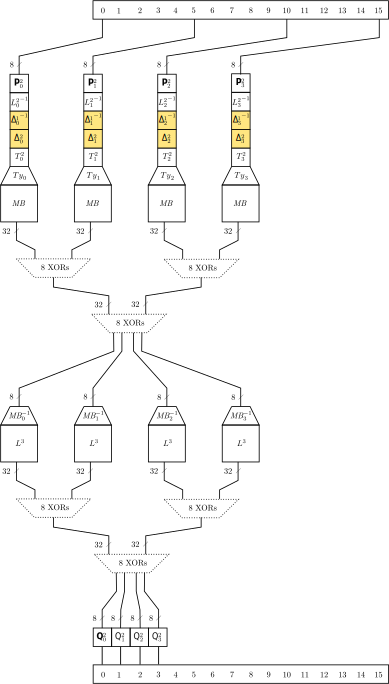
\includegraphics{WBAES_PQ_DUAL.pdf}}}
% \begin{columns}
%      \begin{column}{0.55\textwidth}
% 	\centerline{\scalebox{0.40}{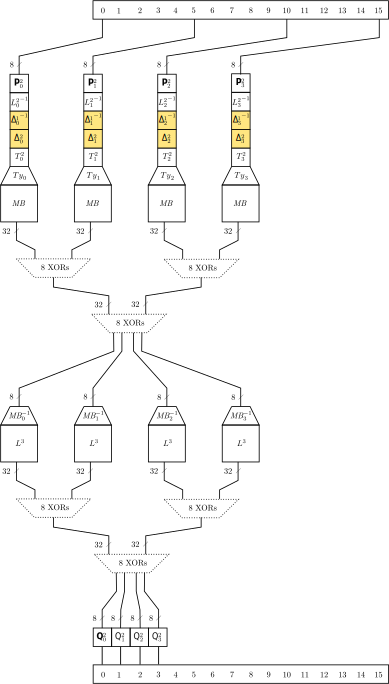
\includegraphics{WBAES_PQ_DUAL.pdf}}}
%      \end{column}
%  
%      \begin{column}{0.45\textwidth}
%  	\begin{figure}
% 	\begin{center}
% 	\leavevmode
% 	\centerline{\scalebox{0.75}{\includegraphics{WBDUAL_closeup.pdf}}}
% 	\end{center}
% 	\end{figure} 
%      \end{column}
%      \end{columns}
\end{frame}

\section{Implementation}
% \begin{frame}
%     \frametitle{Implementation}
%     Implementation    
% \end{frame}

\begin{frame}
    \frametitle{Implementation - whitebox AES scheme}
    \centerline{\scalebox{0.25}{\includegraphics{wbaes_header.jpg}}}
\end{frame}

\begin{frame}
    \frametitle{Implementation - whitebox dual AES scheme}
    \centerline{\scalebox{0.25}{\includegraphics{wbaes_gen.jpg}}}
\end{frame}

\begin{frame}
    \frametitle{Implementation - BGE attack}
    \centerline{\scalebox{0.25}{\includegraphics{wbaes_attack.jpg}}}
\end{frame}

\begin{frame}
    \frametitle{Implementation - BGE attack}
    We then discovered, that BGE attack works also on the whitebox dual AES scheme! (It should not)
    
    \bigskip
    
    \centerline{\scalebox{0.25}{\includegraphics{attack_screen.jpg}}}
\end{frame}

\begin{frame}
    \frametitle{What is wrong with dual AES scheme?}
    \begin{itemize}
     \item BGE attack considers dual AES implementation as a normal ones
     \begin{itemize}
      \item same irreducible polynomial defining field
      \item same generator of the field
     \end{itemize}
     \item so why it works?
     \begin{itemize}
      \item \alert{linear} mapping $\Delta$ transforming one dual AES to another dual AES
      \item \alert<+>{linear} mapping $\Delta$ can be merged with non-linear random bijections
      \item removed in the attack, has \alert{no effect} whatsoever
      \item proof in master thesis
     \end{itemize}
    \end{itemize}
    
    \centerline{\scalebox{0.75}{\includegraphics{WBDUAL_closeup.pdf}}}
\end{frame}

\begin{frame}
    \frametitle{What is wrong with dual AES scheme?}
    { \Fontvi{
    \begin{subequations} \label{eq:wb_dual_aes_r_proof}
	\begin{align} 
	&Q^{r \; \prime}_{i,j}              \left( \bigoplus^3_{l=0} \Delta(\alpha_{l,j}) \cdot \left( \Delta \times A \times \Delta^{-1} \left(               \left(\Delta \circ P^{r \; \prime\prime}_{i,l}\left(x_{i,l}\right) \oplus \Delta\left(k_{i,l}\right) \right)^{-1^{\Delta}\; \gfe} \right) \oplus \Delta \left(c\right) \right) \right) \nonumber \\ 
	&Q^{r \; \prime}_{i,j} \circ \Delta \left( \bigoplus^3_{l=0}        \alpha_{l,j}  \cdot \left(               A \times \Delta^{-1} \left(               \left(\Delta \circ P^{r \; \prime\prime}_{i,l}\left(x_{i,l}\right) \oplus \Delta\left(k_{i,l}\right) \right)^{-1^{\Delta}\; \gfe} \right) \oplus              c        \right) \right) \nonumber \\ 
	&Q^{r \; \prime}_{i,j} \circ \Delta \left( \bigoplus^3_{l=0}        \alpha_{l,j}  \cdot \left(               A \times \Delta^{-1} \left( \left( \Delta \left(             P^{r \; \prime\prime}_{i,l}\left(x_{i,l}\right) \oplus             k_{i,l}\right) \right)^{-1^{\Delta}\; \gfe} \right) \oplus              c        \right) \right) \nonumber \\ 
	&Q^{r \; \prime}_{i,j} \circ \Delta \left( \bigoplus^3_{l=0}        \alpha_{l,j}  \cdot \left(               A \times \Delta^{-1} \left( \Delta        \left(             P^{r \; \prime\prime}_{i,l}\left(x_{i,l}\right) \oplus             k_{i,l}        \right)^{-1\; \gfe} \right)          \oplus              c        \right) \right) \nonumber \\
	&Q^{r \; \prime}_{i,j} \circ \Delta \left( \bigoplus^3_{l=0}        \alpha_{l,j}  \cdot \left(               A \times             \left(               \left(             P^{r \; \prime\prime}_{i,l}\left(x_{i,l}\right) \oplus             k_{i,l}        \right)^{-1\; \gfe} \right)          \oplus              c        \right) \right) \nonumber \\
	&Q^{r \; \prime}_{i,j} \circ \Delta \left( \bigoplus^3_{l=0}        \alpha_{l,j}  \cdot \left(               A \times             \left(               \left(             P^{r \; \prime\prime}_{i,l}\left(x_{i,l}\right) \oplus             k_{i,l}        \right)^{-1\; \gfe} \right)          \oplus              c        \right) \right) \nonumber \\
	&Q^{r \; \prime}_{i,j} \circ \Delta \circ R_{i,j}^{\prime}\left(x_{i,0}, x_{i,1}, x_{i,2}, x_{i,3}\right) \nonumber
	\end{align}
    \end{subequations}}}
\end{frame}

\section{Improvements}
\subsection{Observations from attacks}
\begin{frame}
    \frametitle{Main observations from attacks}
    \begin{itemize}
     \item mostly algebraic attacks
     \item key schedule reversibility is a weakness
     \item attacks use a public knowledge of static building blocks (S-boxes, MixColumns)
    \end{itemize}
    
    \begin{block}{Kerckhoffs's principle}
	According to Kerckhoffs's principle, cipher security should be based on the secrecy of a secret key not the design of the cipher.
    \end{block}
\end{frame}

\subsection{Solutions}
\begin{frame}
    \frametitle{Solutions}
    \begin{itemize}
     \item AES is not suitable for whitebox context (no secure whitebox implementation exists)
     \item design a new cipher for whitebox context
     \item transform key-invariant building blocks to key-dependent
     \begin{itemize}
      \item preserve same security level
      \item add randomness
      \item neglect hardware implementation issues
     \end{itemize}  
    \end{itemize}
    
    \begin{block}{Suggested modifications}
	\begin{itemize}
	 \item non-invertible key schedule
	 \item key-dependent S-boxes
	 \item stronger diffusion layer (larger, key-dependent)
	\end{itemize}
    \end{block}
\end{frame}

\subsubsection{Key schedule}
\begin{frame}
    \frametitle{Key schedule}
    Issues:
    \begin{itemize}
     \item 2 consecutive round keys $\rightarrow$ we obtain all round keys
     \item attack does not need to attack on each round
    \end{itemize}
    
    \bigskip
    Solution:
    \begin{itemize}
     \item use hash function to derive round keys
     \item use expensive hash function (e.g., KPDF2)
     \item whitebox context $\rightarrow$ each round key has 
	   to be considered as a separate, strong encryption key
     \item 
    \begin{equation}\label{eq:keySchedule}
    k_i^r = \left\{ 
    \begin{array}{l l} 
	hash_{N_{bc}, N_{sha}}(key, salt)_i                   & \quad \text{if $r=0$}\\
	hash_{N_{bc}, N_{sha}}(k^{r-1} \; || \;  key, salt)_i & \quad \text{otherwise}
    \end{array} \right.
    \end{equation}
    \end{itemize}
\end{frame}

\subsubsection{S-Boxes}
\begin{frame}
    \frametitle{S-boxes}
    \begin{itemize}
     \item Key-invariant S-Box is used in BGE attack
     \item Use concept of key-dependent S-boxes (Blowfish, Twofish)
    \end{itemize}
    
     \begin{columns}
     \begin{column}{0.50\textwidth}
	Twofish S-boxes
 	\begin{subequations}
	\begin{align}
	    s_{0,k_0,k_1}\left(x\right) &= q_1\left[q_0\left[q_0\left[x\right] \oplus k_0 \right] \oplus k_1 \right] \nonumber \\
	    s_{1,k_2,k_3}\left(x\right) &= q_0\left[q_0\left[q_1\left[x\right] \oplus k_2 \right] \oplus k_3 \right] \nonumber \\
	    s_{2,k_4,k_5}\left(x\right) &= q_1\left[q_1\left[q_0\left[x\right] \oplus k_4 \right] \oplus k_5 \right] \nonumber \\
	    s_{3,k_6,k_7}\left(x\right) &= q_0\left[q_1\left[q_1\left[x\right] \oplus k_6 \right] \oplus k_7 \right] \nonumber
	\end{align}
	\end{subequations}
	Where $q_0, q_1$ are fixed permutations.
     \end{column}
 
     \begin{column}{0.50\textwidth}
 	\begin{figure}
	\begin{center}
	\leavevmode
	\centerline{\scalebox{0.4}{\includegraphics{twofish_core.pdf}}}
	\end{center}
	\caption{Twofish core}
	\end{figure} 
     \end{column}
     \end{columns}
\end{frame}

\subsubsection{Diffusion layer}
\begin{frame}
    \frametitle{Diffusion layer}
    Issues:
    \begin{itemize}
     \item 32 bit diffusion is too small (invertion attack)
     \item $8 \rightarrow 32$ table type II
     \item limitation - HW implementation concerns
     \item low dependency of output on input within one round
     \begin{itemize}
      \item one output byte depends on 4 input bytes (16 in total)
      \item \emph{ShiftRows} effect is negligible in whitebox context
     \end{itemize}
    \end{itemize}
    
    \medskip
    Solutions:
    \begin{itemize}
     \item neglect HW implementation performance
     \item increase diffusion layer on whole round
     \item more possible diffusion layers with same level of security (MDS codes), key dependency
    \end{itemize}
\end{frame}

\begin{frame}
    \frametitle{Diffusion layer}
    \centerline{\scalebox{1.0}{\includegraphics{AES_MDS.pdf}}}
    \centerline{\hbox{\tiny Credit:\thinspace{Jr., Jorge Nakahara and Abrahao, Elcio, \it{A New Involutory {MDS} Matrix for the {AES}}}}}
\end{frame}

\begin{frame}
    \frametitle{Security gain}
    \begin{itemize}
     \item BGE attack is not possible anymore
     \begin{itemize}
      \item naive mounting would require to try all possible key-dependent combinations of building blocks (diffusion, S-Boxes)
      \item no key extraction due to key schedule modification
     \end{itemize}
     \item Inverting the cipher is much more difficult
     \begin{itemize}
	\item function is now too wide
	\item each output byte depends on each input byte within one round
	\item stronger diffusion
     \end{itemize}
     \item our opinion: key-dependency and randomization are important concepts
    \end{itemize}
    
    Drawbacks:
    \begin{itemize}
     \item new cipher $\rightarrow$ need to analyze (statistical) blackbox properties
     \item no backward compatibility
     \item lower throughput, computationally more intensive
     \item increased implementation (tables) size 
    \end{itemize}
\end{frame}


\section{Questions and Discussion}
\subsection{Oponent's question}

\begin{frame}
    \frametitle{Oponent's question}
    \begin{block}{Question}
     Explain the following equation: $\widetilde{Q}(\psi(g)) = g(0), \; g \in \mathcal{S}$
    \end{block}
    \begin{itemize}
     \item It is core of the first part of the BGE attack (recovering non-linear part of IO bijections)
     \item Need to explain whole first part of the attack.
    \end{itemize}
\end{frame}

\subsubsection{BGE attack introduction}
\begin{frame}
  \frametitle{BGE attack}
    \begin{figure}
    \begin{center}
    \leavevmode
    \centerline{\scalebox{1.0}{\includegraphics{BGE_round.pdf}}}
    \end{center}
    \caption{WB AES round from BGE attack perspective, one of $R^r_j,\; j=0,\dots,3$}
    \label{fig:aes_round_bge}
    \end{figure} 

     \begin{equation} \label{eq:y0}    
    \begin{aligned}
    y_0\left(x_0, c_1, c_2, c_3 \right) &= Q^r_{0,j} \left(\alpha T^r_{0,j}\left(P^r_{0,j}\left(x_0\right)\right) \oplus \beta_{c_1,c_2,c_3}\right) \\
				        &= Q^r_{0,j} \circ \oplus_{\beta_{c_1,c_2,c_3}} \circ \alpha \cdot T^r_{0,j} \circ P^r_{0,j} \left(x_0\right)
    \end{aligned}
    \end{equation}
\end{frame}

\begin{frame}
    Fix $c_2 = c_3 = 0$ (WLOG).
    \medskip
     \begin{columns}
     \begin{column}{0.35\textwidth}
 	\centerline{\scalebox{0.8}{\includegraphics{BGE_round.pdf}}}
     \end{column}
 
     \begin{column}{0.55\textwidth}
 	\begin{equation*}
	y_0\left(x_0, c_1\right) = Q^r_{0,j} \circ \oplus_{\beta_{c_1}} \circ \alpha \cdot T^r_{0,j} \circ P^r_{0,j} \left(x_0\right)
	\end{equation*}
     \end{column}
     \end{columns}

      \begin{subequations}
     \begin{align}
     & y_0\left(x_0, b\right) \circ y_0^{-1}\left(x_0, a\right) = \nonumber \\
     &=           \left( Q_{0,j}      \circ \oplus_{\beta_b}                         \circ \alpha \cdot T_{0,j}    \circ P_{0,j}     \right) \nonumber
	\circ     \left( P^{-1}_{0,j} \circ \left(\alpha \cdot T_{0,j}\right)^{-1}   \circ \oplus_{\beta_a}        \circ Q^{-1}_{0,j}\right) \nonumber \\
     &= Q_{0,j} \circ \oplus_{\beta_b} \circ \oplus_{\beta_a} \circ Q^{-1}_{0,j}                                                             \nonumber \\
     &= Q_{0,j} \circ \oplus_{\left(\beta_b \oplus \beta_a\right)} \circ Q^{-1}_{0,j}                                                        \nonumber \\
     &= Q_{0,j} \circ \oplus_{\beta_c} \circ Q^{-1}_{0,j}										     \nonumber
     \end{align}
    \end{subequations}
\end{frame}

\subsubsection{Isomorphism}
\begin{frame}
    \frametitle{Isomorphism}
    \begin{block}{Isomorphism}
    \begin{center}
    \begin{tabular}{ r  c c c }
	\multirow{2}{*}{$\varphi \; :$} & $(\mathcal{S}, \circ )$  & $\longrightarrow$ & $(\gf^8, \oplus)$ \\
	                                & $Q \circ \oplus_{\beta} \circ Q^{-1} $ & $\longmapsto$ & $\left[ \beta \right]$
    \end{tabular}
    \end{center}
    
    \begin{itemize}
     \item $f_1, f_2 \in \mathcal{S}$, then also $f_2 \circ f_1 \in \mathcal{S}$ \pause
     \item $f_2 \circ f_1 = (Q \circ \oplus_{\beta_2} \circ Q^{-1}) \circ (Q \circ \oplus_{\beta_1} \circ Q^{-1}) = Q \circ \oplus_{(\beta_1 \oplus \beta_2)} \circ Q^{-1}$ \pause
     \item $\varphi(f_1 \circ f_2) = \varphi(f_1) \oplus \varphi(f_2)$ \pause
    \end{itemize}

\end{block}
    
    $\varphi$ is isomorphism, but we don't know it.
    \begin{itemize}
     \item we have set $\mathcal{S}$ of functions $f$ of the form $Q \circ \oplus_\beta \circ Q^{-1}$
     \item we don't know $\beta$ for some $f \in \mathcal{S}$
    \end{itemize}
\end{frame}

\begin{frame}
    \begin{block}{Isomorphism}
	\begin{center}
	\begin{tabular}{ r  c c c }
	    \multirow{2}{*}{$\varphi \; :$} & $(\mathcal{S}, \circ )$  & $\longrightarrow$ & $(\gf^8, \oplus)$ \\
					    & $Q \circ \oplus_{\beta} \circ Q^{-1} $ & $\longmapsto$ & $\left[ \beta \right]$
	\end{tabular}
	\end{center}
    \end{block}
    \medskip

    Imagine we know $\beta$: \pause
    \begin{itemize}
     \item Select a tuple $(f_1, \dots ,f_8),\; f_i \in \mathcal{S}$, s.t. $(\varphi(f_1), \dots , \varphi(f_8)) = ([e_i])_{i=1,\dots,8}$ is a standard base of $\gf^8$ \pause
     \item It holds $f_i = Q \circ \oplus_{2^{i-1}} \circ Q^{-1}$, so that $([\varphi(f_i)])_{i=0,\dots,8} = ([e_i])_{i=0,\dots,8} $ \pause
      
     \item Then $(f_1, \dots ,f_8)$ is a base of $(\mathcal{S}, \circ)$, so it holds: \\ 
	    $\forall f \in \mathcal{S}, \exists ! (\varepsilon_1, \dots, \varepsilon_8) \in \{0,1\}^8, \; f = f_8^{\varepsilon_8} \circ f_7^{\varepsilon_7} \circ \cdots \circ f_1^{\varepsilon_1}$  \pause
     \item Then $\varphi(f) = \varphi(f_8^{\varepsilon_8}) \oplus \varphi(f_7^{\varepsilon_7}) \oplus \cdots \oplus \varphi(f_1^{\varepsilon_1})$ \pause
     \item Then $\varphi(f) = [e_8]^{\varepsilon_8} \oplus [e_7]^{\varepsilon_7} \oplus \cdots \oplus [e_1]^{\varepsilon_1}$ \pause
     
     \item But we don't know $\varphi$
     \end{itemize}
\end{frame}

\begin{frame}
\begin{block}{Isomorphism}
    \begin{center}
    \begin{tabular}{ r  c c c }
	\multirow{2}{*}{$\varphi \; :$} & $(\mathcal{S}, \circ )$  & $\longrightarrow$ & $(\gf^8, \oplus)$ \\
	                                & $Q \circ \oplus_{\beta} \circ Q^{-1} $ & $\longmapsto$ & $\left[ \beta \right]$
    \end{tabular}
    \end{center}
\end{block}
\begin{itemize}
 \item Select an \alert{arbitrary} tuple $(f_i)_{i=1,\dots,8}$ that form a base of $\mathcal{S}$ \pause
 \item $(f_i)_{i=1,\dots,8}$ is arbitrary, thus $([\varphi(f_i)])_{i=0,\dots,8} \neq ([e_i])_{i=0,\dots,8} $ in general \pause
 \item $\varphi(f_i) = [\beta_i]$ in general \pause
 \item thus $\varphi(f) = \bigoplus_{i=1}^8 [\beta_i]$, $([\beta_i])_{i=0,\dots,8}$ is \alert{some} base of $\gf^8$ \pause

%  \item We have $(f_i)_{i=1,\dots,8}$, base of $\mathcal{S}$, thus $f = f_8^{\varepsilon_8} \circ f_7^{\varepsilon_7} \circ \cdots \circ f_1^{\varepsilon_1}$ \pause
%  \item Then $\varphi(f) = \varphi(f_8^{\varepsilon_8}) \oplus \varphi(f_7^{\varepsilon_7}) \oplus \cdots \oplus \varphi(f_1^{\varepsilon_1})$
%  \item $\varphi(f_i) = [\beta_i]$, thus $\varphi(f) = \bigoplus_{i=1}^8 [\beta_i]$, $([\beta_i])_{i=0,\dots,8}$ is base of $\gf^8$ \pause
%  \item Ideally $f_i = Q \circ \oplus_{2^{i-1}} \circ Q^{-1}$, so that $([\varphi(f_i)])_{i=0,\dots,8} = ([e_i])_{i=0,\dots,8} $ \pause
%  \item Problem is, we don't know $\beta_i$ for given $f_i = Q \circ \oplus_{\beta_i} \circ Q^{-1}$ \pause
 \item Instead we define $\psi(f_i) = [e_i]$, for some base  $(f_i)_{i=1,\dots,8}$ 
    \begin{itemize}
	 \item $(f_i)_{i=1,\dots,8}$ is standard base of $\mathcal{S}$
	 \item $(\psi(f_i))_{i=1,\dots,8}=([e_i])_{i=1,\dots,8}$ is base of $\gf^8$
    \end{itemize}	  \pause
 \item Then exists (unknown) base change matrix $L$, s.t. $L[e_i] = [\beta_i]$
 \item So we can define $\psi = L^{-1} \circ \varphi$ 
    

\end{itemize}

\end{frame}


\subsubsection{Recovering non-linear parts of IO bijections}
\begin{frame}\frametitle{Commutative diagram}
    \begin{block}{Isomorphism}
    \begin{center}
    \begin{tabular}{ r  c c c }
	\multirow{2}{*}{$\varphi \; :$} & $(\mathcal{S}, \circ )$  & $\longrightarrow$ & $(\gf^8, \oplus)$ \\
	                                & $Q \circ \oplus_{\beta} \circ Q^{-1} $ & $\longmapsto$ & $\left[ \beta \right]$
    \end{tabular}
    \end{center}
    \end{block}
    
    \medskip
    Let's have $f \in \mathcal{S}$. Recall $\psi = L^{-1} \circ \varphi$ \\
    \bigskip
    
    \scalebox{1.2}{\includegraphics{comut_1.pdf}}
\end{frame}

\begin{frame}\frametitle{Commutative diagram}
    \begin{block}{Isomorphism}
    \begin{center}
    \begin{tabular}{ r  c c c }
	\multirow{2}{*}{$\varphi \; :$} & $(\mathcal{S}, \circ )$  & $\longrightarrow$ & $(\gf^8, \oplus)$ \\
	                                & $Q \circ \oplus_{\beta} \circ Q^{-1} $ & $\longmapsto$ & $\left[ \beta \right]$
    \end{tabular}
    \end{center}
    \end{block}
    
    \medskip
    Let's have $f \in \mathcal{S}$. Recall $\psi = L^{-1} \circ \varphi$ \\
    \bigskip
    
    \scalebox{1.2}{\includegraphics{comut_2.pdf}}\\
    $f = Q \circ \oplus_{\varphi(f)} \circ Q^{-1} $
\end{frame}

\begin{frame}\frametitle{Commutative diagram}
    \begin{block}{Isomorphism}
    \begin{center}
    \begin{tabular}{ r  c c c }
	\multirow{2}{*}{$\varphi \; :$} & $(\mathcal{S}, \circ )$  & $\longrightarrow$ & $(\gf^8, \oplus)$ \\
	                                & $Q \circ \oplus_{\beta} \circ Q^{-1} $ & $\longmapsto$ & $\left[ \beta \right]$
    \end{tabular}
    \end{center}
    \end{block}
    
    \medskip
    Let's have $f \in \mathcal{S}$. Recall $\psi = L^{-1} \circ \varphi$ \\
    \bigskip
    
    \scalebox{1.2}{\includegraphics{comut_3.pdf}}\\
    $f = Q \circ \oplus_{\varphi(f)} \circ Q^{-1} = Q \circ L \circ \oplus_{\psi(f)} \circ L^{-1} \circ Q^{-1} $
\end{frame}

\begin{frame}\frametitle{Commutative diagram}
    \begin{block}{Isomorphism}
    \begin{center}
    \begin{tabular}{ r  c c c }
	\multirow{2}{*}{$\varphi \; :$} & $(\mathcal{S}, \circ )$  & $\longrightarrow$ & $(\gf^8, \oplus)$ \\
	                                & $Q \circ \oplus_{\beta} \circ Q^{-1} $ & $\longmapsto$ & $\left[ \beta \right]$
    \end{tabular}
    \end{center}
    \end{block}
    
    \medskip
    Let's have $f \in \mathcal{S}$. Recall $\psi = L^{-1} \circ \varphi$ \\
    \bigskip
    
    \scalebox{1.2}{\includegraphics{comut_4.pdf}}\\
    $f = Q \circ \oplus_{\varphi(f)} \circ Q^{-1} = Q \circ L \circ \oplus_{\psi(f)} \circ L^{-1} \circ Q^{-1} $
\end{frame}

\begin{frame}\frametitle{Commutative diagram}
    \begin{block}{Isomorphism}
    \begin{center}
    \begin{tabular}{ r  c c c }
	\multirow{2}{*}{$\varphi \; :$} & $(\mathcal{S}, \circ )$  & $\longrightarrow$ & $(\gf^8, \oplus)$ \\
	                                & $Q \circ \oplus_{\beta} \circ Q^{-1} $ & $\longmapsto$ & $\left[ \beta \right]$
    \end{tabular}
    \end{center}
    \end{block}
    
    \medskip
    Let's have $f \in \mathcal{S}$. Recall $\psi = L^{-1} \circ \varphi$ \\
    \bigskip
    
    \scalebox{1.2}{\includegraphics{comut_5.pdf}}\\
    $f = Q \circ \oplus_{\varphi(f)} \circ Q^{-1} = Q \circ L \circ \oplus_{\psi(f)} \circ L^{-1} \circ Q^{-1} = \widetilde{Q} \circ \oplus_{\psi(f)} \circ \widetilde{Q}^{-1}$
\end{frame}

\begin{frame}\frametitle{Commutative diagram}    
    \centerline{\scalebox{1.2}{\includegraphics{comut_5.pdf}}}
    \bigskip
    
    \begin{itemize}
     \item Define $A(x) = L(x \oplus (Q \circ L)^{-1}(['00'])) = L(x) \oplus Q^{-1}(['00'])$
     \item Define $\widetilde{Q} = Q \circ A$
     \item $f = Q \circ \oplus_{\varphi(f)} \circ Q^{-1} = Q \circ L \circ \oplus_{\psi(f)} \circ L^{-1} \circ Q^{-1} = \widetilde{Q} \circ \oplus_{\psi(f)} \circ \widetilde{Q}^{-1}$
    \end{itemize}
\end{frame}


\begin{frame}\frametitle{Commutative diagram}    
    \centerline{\scalebox{1.2}{\includegraphics{comut_5.pdf}}}
    \bigskip
%     \begin{frame}{Frame 1}
    \begin{itemize}
     %\item $\widetilde{Q}^{-1}('00') = ['00']$
    \item Observe $\widetilde{Q}^{-1}('00') = Q(L(0) \oplus Q^{-1}(['00'])) = Q(Q^{-1}(['00'])) = ['00']$\\
	$L$ is linear (unknown), $A$ defined in this way so this holds (artificial)! \pause
     \item $f = Q \circ \oplus_{\varphi(f)} \circ Q^{-1} = \widetilde{Q} \circ \oplus_{\psi(f)} \circ \widetilde{Q}^{-1} $, from commutative diagram \pause
     \item $f('00') = \widetilde{Q}( \psi(f) \oplus \widetilde{Q}^{-1}('00')) = \widetilde{Q}( \psi(f) )$ \pause
     \item Observe $\widetilde{Q}^{-1} \circ Q = A^{-1}$ 
    \end{itemize}
%     \end{frame}
\end{frame}

\subsection{Questions}
\begin{frame}
  \begin{center}
    Questions?
  \end{center}
\end{frame}

\begin{frame}
  \begin{center}
    Thank you for your attention
  \end{center}
\end{frame}

\end{document}

